\documentclass[12pt,a4paper]{article}
\usepackage[utf8]{inputenc}
\usepackage{amsmath}
\usepackage{amsfonts}
\usepackage{amssymb}
\usepackage{dsfont}
\usepackage{wrapfig}
\usepackage{graphicx}
\usepackage{pgf, tikz}
\usepackage[left=2cm,right=2cm,top=2cm,bottom=2cm]{geometry}

\title{Single Item Lot Sizing}
 \date{}
\begin{document}
	\maketitle
	
	\section*{Présentation}
	
	\paragraph{Problématique} Nous proposons $N$ types d'objets. Discrétisons un intervalle de temps en $T$ périodes. Nous disposons d'une machine ne pouvant produire qu'un seul type d'objets par période. \medbreak De plus, à chaque période $t$, nous devons satisfaire une demande $d_{it}$ en objets de type $i$, initialiser la machine ce qui implique un coût $f_{it}$ si nous souhaitons produire des objets de type $i$ et payer un coût de production $p_{it}$ pour chaque objet de type $i$ produit.
	
	\paragraph{Variables}
	Posons $x_{it}$ la quantité d'objets de type $i$ produit à la période $t$. \medbreak Posons $y_{it} = \left\lbrace \begin{aligned}
	1 ~& \text{si nous produisons des objets de type }i \text{ à la période } t \\
	0 ~& \text{sinon}
\end{aligned}	 \right.$.

 	\paragraph{Modélisation} Nous ne considérons pas les coûts de stockage. Nous pouvons les prendre en compte grossièrement dans les coûts de production. Par exemple, des coûts de production décroissants de période en période. En effet, si nous produisons en première période, nous pouvons être amenés à stocker plus longtemps qu'en produisant dans les dernières périodes.
 	
 	$$ [P] ~~~ min \sum_{t=1}^{T} \sum_{i=1}^{N} p_{it}x_{it} + f_{it} y_{it} $$ 		
 	
	\begin{eqnarray}	
 		\sum_{\tau=1}^{t} x_{i \tau} &\geq d_{it}, & \forall t \in \{1,T\} ~ \forall i \in \{1,N\} \\
 		x_{it} &\leq d_{it}y_{it}, & \forall t \in \{1,T\} ~ \forall i \in \{1,N\} \\
 		\sum_{i=1}^{N} y_{it} &\leq 1, & \forall t \in \{1,T\} \\
 		x_{it} \geq 0,& y_{it} \in \{0, 1\} &  \forall t \in \{1,T\} ~ \forall i \in \{1,N\} \nonumber
 	\end{eqnarray}	
 	
 	\newpage
 	
	\section*{Décomposition de Dantzig-Wolfe}
	\subsection*{Sous problème}
	\paragraph{Présentation} Nous savons résoudre le problème $[P]$ sans la contrainte $(3)$, c'est-à-dire en ayant une machine pouvant produire plusieurs types d'objets à chaque période. Pour représenter ce sous-problème $[SP]$, considérons un graphe G, chaque sommet représentant une période et chaque arête $(u,v)$ le coût pour couvrir la demande $D^i_{u,v} = \sum_{j=u+1}^{v} d_{ij}$ en objets de type $i$. \medbreak
	
	\begin{figure}[h!]
		\centering
		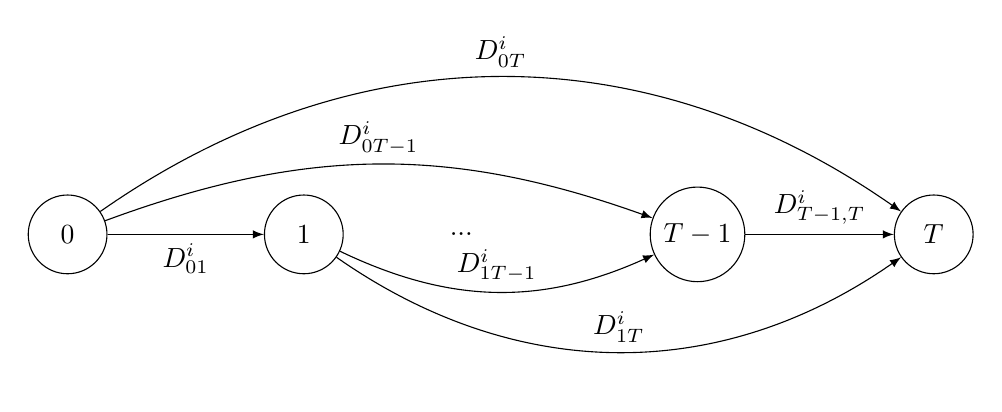
\begin{tikzpicture}
         \node[draw,circle,minimum size=1.0cm](A) at (0,0) {$0$};
         \node[draw,circle,minimum size=1.0cm](B) at (3,0) {$1$};
         \node[](H) at (5,0){...};
         \node[draw,circle,minimum size=1.0cm](C) at (8,0) {$T-1$};
         \node[draw,circle,minimum size=1.0cm](D) at (11,0) {$T$};

         \draw[->,>=latex](A) -- node[midway,below]{$D^i_{01}$} (B);
         \draw[->,>=latex](A)to[bend left=20] node[midway,above]{$D^i_{0T-1}$} (C);
         \draw[->,>=latex](A)to[bend left=35] node[midway,above]{$D^i_{0T}$} (D);
         \draw[->,>=latex](B)to[bend left=-25] node[midway,above]{$D^i_{1T-1}$} (C);
         \draw[->,>=latex](B)to[bend left=-35] node[midway,above]{$D^i_{1T}$} (D);
         \draw[->,>=latex](C) -- node[midway,above]{$D^i_{T-1,T}$} (D);
		\end{tikzpicture}
	\caption{Graphe pour résoudre le sous-problème pour les objets de type $i$.}
	\end{figure}
	
	 Pour chaque objet de type $i$, nous souhaitons calculer dans le graphe de la figure 1, le chemin de coût minimum.
	 
	 \paragraph{Résolution} Soit $M(i,a,b)$ le coût minimum pour couvrir la demande en item $i$ de la période $a$ à la période $b$.
	 
	 $$ M(i,a,b) =  \min_{l \in \{a,b\}} \{ p_{al}D_{al} + M(i,l,b) \} $$
	 
	 On peut donc résoudre le problème $[SP]$.
	 
	 $$ OPT([SP]) = \sum_{i=0}^N min~M(i,0,T) $$
	
	Nous notons $Z$ l'ensemble des points extrêmes générés de $[SP]$, $Z=\{z^q\}_{q\in Q} = \{ (g^q~h^q) \}_{q\in Q}$.
	
\subsection*{Décomposition}
\paragraph{Maître restreint} Soit le problème restreint $[M^t]$ obtenu par la décomposition de $[P]$
 	$$ [M^t] ~~~ min \sum_{q \in Q^t} (p~f)^T(g^q~h^q)\lambda_q $$	
 	
	\begin{eqnarray}	
 		\sum_{q \in Q^t} \lambda_q \sum_{i=1}^N h_{i\tau}^q &\leq 1, & \forall \tau \in \{1,T\} \\
 		\sum_{q \in Q^t} \lambda_q &=1 & \\
 		\lambda_q \geq 0,& q \in Q^t & \nonumber
 	\end{eqnarray}
 	
\newpage 
\paragraph{Dual de $[M^t]$} Soient $\pi$ variable duale de la contrainte $(4)$ et $\eta$ variable duale de la contrainte $(5)$.

$$ [DM^t] ~~~ max ~ \eta $$	

\begin{eqnarray}	
 		\sum_{\tau=1}^T \pi_{\tau} \left( \sum_{i=1}^N h_{i\tau}^q -1 \right) + \eta &\leq (p~f)(g^q~h^q)^T  &, q\in Q^t\\
 		\pi \in \mathbb{R}^T_+,& \eta \in \mathbb{R}^1 \nonumber
 \end{eqnarray}
 	

\section*{Résolution}	

\paragraph{Initialisation} Trions les types objets tels qu'un ensemble d'objets est de type $i$ si $\forall \tau < i , d_{i\tau} = 0$. Ainsi, pour les objets de type $i$, la première période à laquelle la demande est non nulle est la période $i$. \medbreak
 Il existe une solution réalisable triviale au problème $[SP]$, ne violant pas la contrainte $(3)$ de $[P]$. Elle consiste, pour les objets de type $i$, à produire à la période $i$ l'ensemble de la demande.
 
 $$ g^0=(\underbrace{D^1_{0T}~0~..~0}_{N \text{ items}} ~ \underbrace{0~D^2_{1T}~..~0} ~ \underbrace{0~0~..~D^N_{N-1,T}} ~0~..~0) $$ 
 
 $$h^0=(\underbrace{1~0~..~0}_{N \text{ items}} ~ \underbrace{0~1~..~0} ~ \underbrace{0~0~..~1} ~0~..~0) \text{ et } \pi^0=(0)_{1 \leq t T} $$
 
 Enfin, nous initialisons la variable $t \leftarrow 1$, indiquant le nombre d'itérations, la borne inférieure $\hat{L}$ et la borne supérieure $\hat{U}$ de $[DM]$.
 
 \paragraph{Solution duale} En appliquant l'algorithme du volume, nous calculons $\pi^{t}$. Posons $x^t$ la solution de $[M^t]$ et $\hat{\pi}$ la meilleure solution duale (correspondant à $\hat{L}$).
 $$\varrho \leftarrow  \dfrac{\hat{U}-L^{t-1}}{\underbrace{\sqrt{\sum_{\tau=1}^T  
 |1 - \sum_{i=1}^N h_{i \tau}^{t-1}|^2 }}_{\parallel \mathds{1} - Ah^{t-1} \parallel}} \times \dfrac{1}{\underbrace{\sqrt{\sum_{\tau=1}^T |1 - \sum_{i=1}^N y_{i \tau}^{t-1}|^2 }}_{\parallel \mathds{1} - Ay^{t-1} \parallel}}$$
 
 Nous pouvons calculer le nouveau vecteur.
 $$ \pi^t_\tau \leftarrow (\hat{\pi}_\tau + \theta \varrho (1-\sum_{i=1}^Ny^{t-1}_{i\tau}))^+ ~~~~ \theta \in [0,2] $$
 
 \paragraph{Oracle} Lagrangian subproblem oracle call
 
 $$ z^t \leftarrow arg\min_{(x~y)\in Z}\{ r^t \leftarrow px^T +  \sum_{\tau=1}^T \sum_{i=1}^N ( f_{i\tau} - \pi_{\tau}^t y_{i\tau}) \}$$
 
 $$L^t \leftarrow r^t + \sum_{\tau=1}^T \pi_{\tau}^t$$
 
 \paragraph{Optimalité pour $[P]$ } Si $z^t$ vérifie la condition $(3)$ et $\pi^t(\mathds{1} - Ah^t)= 0$.
 
 \paragraph{Actualisation meilleure solution duale} Si $L^t > \hat{L}$ alors $\hat{\pi}\leftarrow \pi^t$ et $\hat{L} \leftarrow L^t$.
 
 \paragraph{Optimalité pour $[LD]$} Il faut vérifier $\hat{L} = \hat{U}$.
 
 \paragraph{Solution primale} Méthode du volume
 $$(x~y)^t \leftarrow \alpha (x~y)^{t-1} + (1- \alpha)(g~h)^t$$
 
 \paragraph{Itération}Nous itérons, $t \leftarrow t+1$ et $Q \leftarrow Q \cup  \{(g~h)^t\}$.
 
 
 \section*{Résultats}
 
 
\end{document}
	